%- THESIS.TEX
%-
%- An example file on how to use vthesis.cls
%- Vassilis Dimakopoulos, 1995 & 1996
%-
%- Use it as you would use report.sty (or .cls).
%-
%- The differences/additions are:
%   - the page layout is set according to Uvic Dec. 1994 rules
%-  - the construction of the `special' pages (titlepage, abstract,
%-       withhold form, etc) is automatic
%-  - the numbering (arabic & roman) of pages is also automatic
%-  - there are aesthetic changes (I call them improvements :-) to
%-       page headers, figure and table captions, etc.
%-  - a few simple entities have been defined
%     o  A \begin{proof} ... \end{proof} environment
%     o  Two simple lists: alphalist and numlist. numlist
%-       (\begin{numlist} \item .. \end{numlist}) is the same
%-       as `enumerate' but puts the numbers in boldface which
%-       looks good to me. Same goes for alphalist but instead of
%-       numbers you get (a), (b), etc.
%-
%- Please double check with the official thesis guidelines.
%- Report problems/questions to dimako@ece.uvic.ca
%-

\documentclass[12pt]{vthesis}   %- If no size given, 11pt is the default
                                %- Uvic now accepts as low as 10pt
\bibliographystyle{ieeetr}

\usepackage{graphics}           %- Or whatever else you need
\usepackage{graphicx}
\usepackage{epsfig}
\usepackage[dvips]{color}

\usepackage[numbers]{natbib}
\graphicspath{ {images/} }

%-----------------------------------------------------
%- Start the text already
%-----------------------------------------------------
\begin{document}

%-
%- Numbering is automatic: arabic & roman page numbers are put in the
%- appropriate pages. Roman paging starts at the first \chapter command.
%-

%-----------------------------------------------------
%- Stuff needed for title page and for other pages too
%-----------------------------------------------------

%\thesistype{Dissertation}       %- If not used, it defaults to "Thesis"
\thesistitle{TOWARDS UNDERSTANDING DIGITAL INFORMATION DISCOVERY}  %- Use capital letters
\name{ELENA VOYLOSHNIKOVA} %- Candidate's name, uppercase is good
\degree{Master of Science}    %- What you're after

%-
%- If you are in a department other than ECE, use the command
%- \department{..}, e.g.
%-
\department{Department of Computer Science}


%- Here give previous degrees

%\prevdegree{M.A.Sc, University of Victoria, 1992}
\prevdegree{B.Sc., University of Victoria, 2002}

%- Let latex know about the committee members,
%-    in the order you want them

\committeemember{Dr.~******, Supervisor,\\ Dept.~of
Computer Science} \committeemember{Dr.~******, Member,\\
Dept.~of Computer Science} \committeemember{Dr.~******,
Member,\\ Dept.~of Computer Science}
\committeemember{Dr.~********, External Examiner}

%- Let latex know the supervisor's name

\supervisor{Dr.~Margaret-Anne Storey}

%-
%- NOW, make the title page
%-

\maketitlepage

%-----------------------------------------------------
%- Do your abstract as normal
%-----------------------------------------------------

\begin{abstract}
Everyday life revolves around the discovery and curation of digital information. People search the Web continuously, from quickly looking up the information needed to complete a task, to endlessly searching for inspiration and knowledge. A variety of studies have modeled information seeking strategies and characterized information seeking and curation activities on the Web. However, there is a lack of research on how existing Web applications support the discovery and management of information, especially concerning the motivations behind them and how different approaches can be compared.

In this paper, we present a study of information discovery tools and how they relate to the nature of information seeking. We propose a conceptual framework that deals with the opportunistic and purposeful aspects of how people discover and manage digital information. This framework can be used when designing, evaluating or updating Web applications.
\end{abstract}

%--------------------------------------------------------------
%- Add table of contents, list of figures, tables etc as normal
%--------------------------------------------------------------

\tableofcontents
\listoffigures
\listoftables


%--------------------------------------------------------------
%- Here is how to add three (optional) pages
%- If you do not like what you get, do it manually
%--------------------------------------------------------------

%\begin{notation}
%\end{notation}

\begin{acknowledgement}
\end{acknowledgement}

\begin{dedication}
\end{dedication}

%--------------------------------
%- From now on you're on your own
%--------------------------------

%
\chapter{Introduction}
\label{chapter:chapter_intro}

Web technologies help people satisfy their information needs. People research their interests and hobbies using various online resources, shoppers search online stores for product characteristics to make purchasing decisions, and travelers visit online booking sites to find information about flights and hotels. In order to accommodate diverse and evolving user needs, Web applications continuously introduce new features and services, empowering information discovery and curation. 

The term ``information discovery'' has been used by many researchers to define or explain various information behaviour paradigms, such as information exploration~\cite{waterworth1991model} and serendipitous information seeking~\cite{foster2003serendipity}. However, the definition of information discovery itself is difficult to articulate. 

Lynch describes resource discovery as a complex collection of activities ranging from locating a well-specified information to iterative research activities, that can involve the identification
of potentially relevant resources, organization and ranking of resources, and resource exploration~\cite{lynch1995networked}. Proper and Bruza apply the term ``information discovery'' in the context of  the identification and retrieval of relevant information from electronic sources~\cite{proper1999information}. 

In the field of cognitive psychology, Jerome S. Bruner~\cite{bruner1961act} defines information discovery as ``all forms of obtaining knowledge for oneself by the use of one's own mind.'' I build on Bruners's definition to underline the importance of the cognitive processes that govern information discovery. Therefore, I consider \textit{information discovery} as a process of obtaining knowledge from digital sources that can involve complex mental tasks and information behavior.  

Information behavior refers to the totality of ways in which humans interact with information~\cite{wilson2000human}. It can enable and support information discovery when targeted at information maintenance and augmentation. This type of information behavior is also known as \textit{digital curation}.

Similar to the term ``information discovery'', the term "digital curation" is perceived differently across disciplines and among researchers. In this thesis, I use the definition proposed by Giaretta~\cite{giaretta2006dcc} and adopted by the Digital Curation Centre\footnote{The Digital Curation Centre is a UK-based organization established to support expertise and practice in digital curation and preservation across communities of practice.} which states that digital curation is a process of maintaining and adding value to an existing body of information to improve its future use and retrieval.   

Information discovery can take on many forms. Web users might be hoping to find particular pieces of information, such as show times and phone numbers, to satisfy specific information needs~\cite{proper1999information}. Alternatively, they might be lacking well-articulated information needs, so they engage in opportunistic browsing~\cite{lindley2012s}. Sometimes people discover information online without even looking for it~\cite{bates1986exploratory}. The nature of information discovery can vary, and therefore, it requires elaborate tool support. The functionality required for information discovery and curation can also be distributed among multiple applications, which often leads to tools that provide integrated solutions. With people having such diverse information needs and methods of looking for information, designing for information discovery is a challenging task~\cite{conaway2010designing, marchionini2006exploratory}.

My research goal is to gain an understanding of how existing tools support digital information discovery and curation addressing the problem of designing Web applications for information discovery. While several researchers propose frameworks targeted at designing information discovery systems~\cite{proper1999information, kerne2004information}, the importance of information curation in the realm of information discovery has been largely overlooked despite the rapidly increasing popularity of socially-curated information spaces. Moreover, much of the existing work that focuses on how people look for and discover information online~\cite{bates1986exploratory, choo2000information, ellis1989behavioural, kellar2006goal, lindley2012s, morrison2001taxonomic, sellen2002knowledge} fails to examine concrete features of existing Web-based information discovery applications that empower real-world users. More research is necessary to determine how different tools and their features provide fundamental support for information discovery and curation.

To enhance information seeking and curating experiences and support users' interactions, I extend existing research by (1) deriving factors that enable information discovery and curation and relating them within a framework, (2) using the framework to establish a set of questions that can be used when evaluating and designing new applications, (3) iteratively evaluating the framework by using it to study and describe current Web applications as well as to design a new application, which in turn helped refine the framework of factors and questions, and (4) relating the framework to user information discovery and curation goals that drive the underlying usage of many Web-based applications. 

This thesis is organized as follows. My methodology and the process of building and refining a conceptual framework is documented in Chapter~\ref{chapter:methodology}. Chapter~\ref{chapter:chapter_related_work} highlights some of the studies and technologies related to information discovery and curation tasks. Chapter~\ref{chapter:old_framework} describes preliminary attempts at building the conceptual framework and outlines their shortcomings. Chapter~\ref{chapter:framework} outlines the conceptual framework and questions that enable digital information discovery and support curation, including specific examples from real-world Web applications. In Chapter~\ref{chapter:evaluation}, I illustrate the framework validation process, demonstrate how the framework can be used to reveal missing features in tools, and propose new directions for development with relation to user goals. I then showcase how the framework can be used for Web application design in Chapter~\ref{chapter:application}. Chapter~\ref{chapter:implications} summarizes the implications for research and practice. This is followed by future work and conclusions in Chapter~\ref{chapter:future_work}.




 
\chapter{Methodology}
\label{chapter:methodology}

The methodology used for the study presented in this thesis consisted of five major steps. To gain a deeper understanding of the problem of information discovery and curation, (1) I conducted a extensive literature review. Based on the literature review, (2) I derived a preliminary set of information discovery and curation design factors and related them within a framework. (3) The framework was then applied for the evaluation of 20 different information discovery applications and iteratively refined after every evaluation. (4) The resulting framework was used to develop a novel place photo discovery application,revealing unforeseen gaps that were consequently addressed. Lastly, (5) the framework was applied to a reevaluation of some of the previously evaluated tools with the purpose of validating its effectiveness.  A summary of the methodology is presented in Figure~\ref{fig:methodology}.
\begin{figure}[ht!]
	\noindent
	\centering
    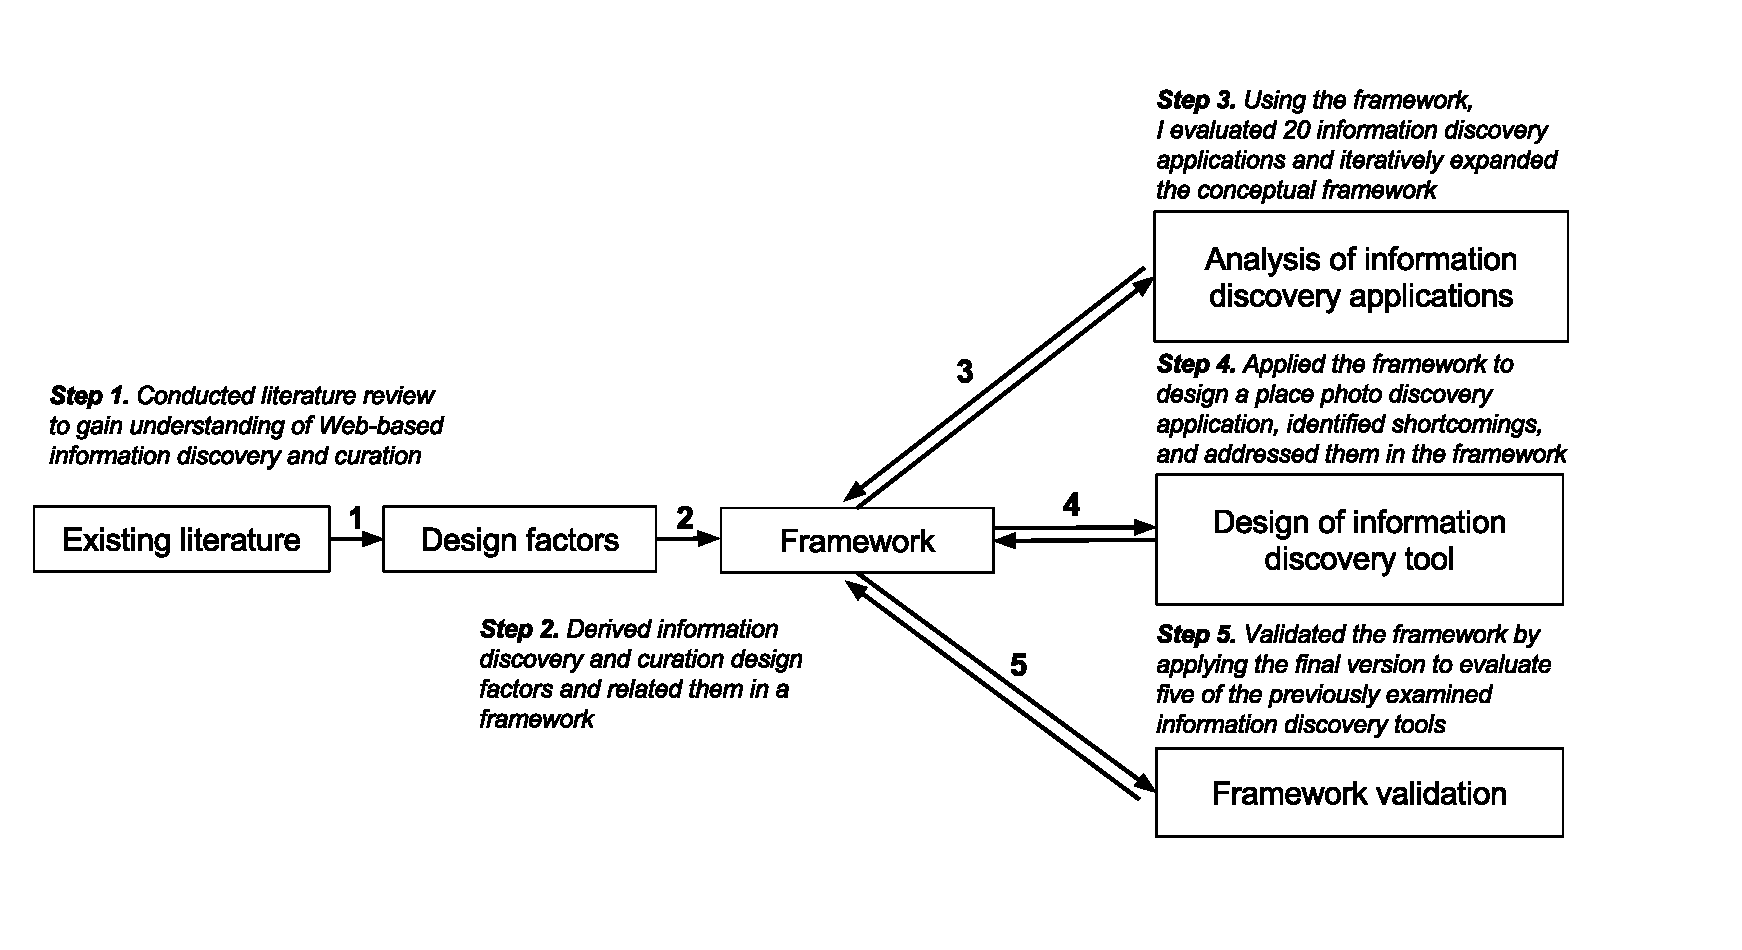
\includegraphics[width=\linewidth]{methodology.pdf}
	\caption{Methodology Overview}
	\label{fig:methodology} 
\end{figure}

{\section{Research Questions and Objective}
This study was designed to address the problem of designing Web applications for information discovery and was motivated by the following research questions and a research objective:

\emph{RQ1:~How do existing Web applications support information discovery?}

\emph{RQ2:~How do existing information discovery applications support information curation?}

\pagebreak 

To address RQ1 and RQ2, I conducted an extensive literature review (see Section~\ref{section:lit_review}) and a case study of 20 information discovery tools (see Section~\ref{section:building}). Using insights from RQ1 and RQ2, I established my main research objective, which is \emph{\textbf{to develop a framework for performing summative and formative evaluation of Web-based information discovery and curation tools}}. I further address my methodology for building the conceptual framework in Sections~\ref{section:building}, \ref{section:applying}, and \ref{section:validating}.

}% end section

{\section{Literature Review}
\label{section:lit_review}
The development of the framework began with an extensive literature review. A diverse set of topics contributed to forming an understanding of information discovery and curation, including information behaviour and information seeking models, high-level Web tasks and modes of Web use, exploration-based models of discovery, and methods of personal and social curation. From this review, the preliminary design factors for the framework were derived. Key findings in the current literature are presented in Chapter~\ref{chapter:chapter_related_work}.
}% end section

{\section{Building and Refining the Conceptual Framework}
\label{section:building}
Through a careful analysis of 20 information discovery applications (see Table~\ref{table:tools}), the framework was iteratively expanded by adding new concepts and establishing relations between those concepts.  The framework was refined as I explored the literature and available tools, and for presentation purposes in this thesis, I present only two versions of the framework. The preliminary framework was a result of this tool analysis and depicted in Chapter~\ref{chapter:old_framework}. The final version of the framework (see Chapter~\ref{chapter:framework}) was a result of developing an information discovery application based on the preliminary work.    

For my case study, I selected some of the most used information discovery applications today and considered the full range of features in those tools (both by referring to the literature and documentation on those tools, as well as exploring the features). The popularity of information discovery applications was determined using Website popularity ranks provided by Alexa\footnote[1]{Alexa is available at www.alexa.com}, a commercial Web traffic data provider. The focus was on applications that had strong information discovery components and lesser priority was given to applications whose purpose revolved only around curation.

I used Yin's strategies for designing a case study~\cite{yin2014case} for guidance. The motivation behind choosing a case study over other methods of qualitative research was based on my choice of research questions, the lack of control over existing applications and their development, and having to focus on contemporary use of real-life Web applications. According to Yin~\cite{yin2014case}, a case study would be an optimal research strategy given the above characteristics.

My study consisted of 20 cases, whereby each case is a Web application that focuses on the support of information discovery. I examined the overall purpose of each application, its description as defined within the application, as well as literature and documentation related to the application (if they were available) against the features that the application provided. For example, if an application provided bookmarking features, I checked if it was indeed intended to be used for information preservation. 

Consequently, the methodology was an iterative process of selecting cases, analyzing them, and determining whether they could be described and evaluated using the framework. If I found a key feature that could not be described, I adapted the framework according to the findings. I repeated the process of case selection and evaluation until the framework was usable for all cases. I then grouped the elements of the framework into categories, recording corresponding questions to ask in order to evaluate applications. 

A list of the tools that were used in this study are presented in Table~\ref{table:tools}. Summaries of their evaluations using the preliminary framework can be found in Appendix~\ref{chapter:appendix_tools}. Other tools were considered throughout the study, however, only the 20 applications presented underwent systematic examination. 

\begin{table*}[htbp]
\small
\caption{Web-based Information Discovery and Curation Tools as of May 15, 2014}
\label{table:tools} 

\begin{tabular}{|p{0.20\linewidth}| p{0.30\linewidth}| p{0.45\linewidth}|}

\hline
\textbf{Application} & \textbf{Address} & \textbf{Description}
\\
\hline
Pinterest       & www.pinterest.com 	& Visual discovery tool \\
\hline
Delicious       & delicious.com 		& Social bookmarking service \\
\hline
Tumblr          & www.tumblr.com 		& Microblogging platform \\
\hline
StumbleUpon     & www.stumbleupon.com  	& Web page discovery tool \\
\hline
Wikipedia       & en.wikipedia.org   	& Free content Internet encyclopedia\\
\hline
Google Maps     & www.google.ca/maps  	& Web mapping service\\
\hline
Rotten Tomatoes & www.rottentomatoes.com & Movie and TV database\\
\hline
500px           & 500px.com            	& Photography site\\
\hline
BucketList      & bucketlist.org  		& Goal tracking and discovery service\\
\hline
We Heart It     & weheartit.com 		& Visual discovery tool \\
\hline
Scoop.it!       & www.scoop.it 			& Online publishing platform \\
\hline
Google Images   & images.google.com  	& Image discovery service \\
\hline
Vimeo           & vimeo.com  			& Video sharing Website\\
\hline
LifeHacker      & lifehacker.com        & Daily blog \\
\hline
YouTube         & www.youtube.com 		& Video hosting platform \\
\hline
Yelp            & www.yelp.ca  			& Business review site\\
\hline
IMDb            & www.imdb.com  		& Movie database \\
\hline
Trip Adviser    & www.tripadvisor.ca 	& Travel site \\
\hline
Urban Spoon     & www.urbanspoon.com    & Online bar and restaurant guide\\
\hline
Thesaurus       & thesaurus.com         & Online thesaurus \\
\hline
\end{tabular}
\end{table*}
} % end section
\pagebreak
{\section{Applying the Framework to the Design of an Information Discovery and Curation Application}
\label{section:applying}

In order to analyze the framework's capabilities when designing for information discovery and curation, I used the framework as a guide for developing a place photo discovery application. The motivation for choosing a place photo discovery application was based on the gaps that were exposed during analysis of some of the applications, such as Google Maps and Pinterest. Applying the framework to designing an application has triggered more changes within the framework, its further extension and refinement. The resulting application is discussed in Chapter~\ref{chapter:application}.
}% end section

{\section{Framework Validation}
\label{section:validating}
In order to further validate the framework, it was applied to the reevaluation of five of the previously examined tools for comparison purposes (see Chapter~\ref{chapter:application}). For each tool, I identified gaps and proposed directions for future development. 
}% end section

{\section{Limitations}
The case study I conducted has a number of limitations. A lack of documentation, research literature, and formal descriptions of available features for some applications introduces a threat to the construct validity of the study. In addition, information discovery tools and features can be used in unintended or unforeseen ways by designers and developers. Therefore, the recorded use of some features within information discovery applications was recorded on my interpretations. To compensate for such limitations, I personally employed the tools over an extended period of time to gain a deeper understanding of their use. In addition, I considered some cases with similar functionality and design to be able to validate or clarify prior findings. 

Many Web applications evolve rapidly. Therefore, my tool analysis only applies to tools at the moment of the study. Additionally, framework validation was performed on five of the previously examined tools, introducing another limitation to the study. 
\pagebreak

Only Web applications running in browsers on a desktop computer were considered in this study. The study can be extended with use of various devices, such as smartphones and tablets, as information discovery patterns and mechanisms may vary for different platforms. 

Another limitation was the lack of prior research on the subject matter. Some researchers have studied information seeking models and high-level Web tasks, but there is a lack of literature on how to enable and support different Web tasks. This opens up opportunities for future research to analyze methods of developing and building frameworks for facilitating and evaluating tools that support other Web tasks, such as communication, transactions, and goal realization.


} % end section


\chapter{Related Work}
\label{chapter:chapter_related_work}

{\section{\sloppy Web-based Information \\Discovery and Curation}

Several researchers have studied various aspects of Web-based information discovery. To gain an understanding of how current Web tools support information discovery and curation, we first studied known characteristics of information-related Web usage, including high-level Web tasks, information seeking behavior, information curation, collaboration in information seeking, and modes of Web use.  

{\subsection{Web Tasks}

Kellar et al. ~\cite{kellar2006} separated Web tasks into five categories: transactions, browsing, fact finding, information gathering, and other uncategorized tasks, with information seeking being composed of browsing, fact finding, and information gathering. Although the authors categorized information gathering as part of information seeking, it is in fact more closely related to digital curation ~\cite{beagrie, wittaker}. In their later work, Kellar et al. ~\cite{kellar2007} added communication and maintenance as additional Web tasks. 

Similarly to Kellar et al., Sellen et al. ~\cite{sellen} identified six tasks that are commonly performed by Web users: browsing, finding, housekeeping, information gathering, communicating, and transacting. Therefore, Kellar et al. and Sellen et al. both identified browsing, fact finding, and information gathering as information-related tasks that users perform online.   

People often engage in information seeking activities to close some knowledge gap that occurred as a result of not having enough information to perform a task ~\cite{proper}. Therefore, when providing tool support for various information discovery tasks, it is useful to consider the motivation behind these tasks as it can be different for each task. Morrison et al. ~\cite{morrison} make a distinction between methods of Web use and purposes. The authors derived a purpose-based taxonomy of Web use, including three purposes or motivations: finding information, comparing pieces of information or choosing products to make a decision, and using the Web to find relevant information to gain an understanding of some subject. Consequently, methods of finding information identified by Morrison et al. are collecting, finding, exploring, and monitoring. The differences between the two taxonomies suggest that different information seeking tasks may be performed to satisfy more than one information seeking purpose. Therefore, each purpose may require more than one task-supporting mechanism. 

Morrison et al. also draws distinction between finding or looking up information and exploratory search. Whereas information lookup involves tasks such as fact retrieval, navigation, and verification, exploration is more cognitively demanding and involves learning and investigation ~\cite{marchionini}. Learning and investigation can be performed over multiple iterations, and can involve learning though various media, "social searching", and serendipitous browsing performed with the goals of knowledge acquisition, socialization, forecasting, and planning.  

} % end subsection

{\subsection{Information Behavior Models}

A number of researchers have proposed models of information seeking and information behavior. Wilson ~\cite{wilson1999} summarized some of the key work ~\cite{ellis1989, dervin, kuhlthau, wilson1997, wilson1981} on information behavior and proposed a new model. According to Wilson's original model of information behavior ~\cite{wilson1981}, information seeking behavior results form the user trying to satisfy their perceived information need. Consequently, the user makes demands on information systems. Success or failure of such demands dictates whether the process is repeated or, if the information need is satisfied, used or communicated with other people. In addition, Wilson defined possible barriers that can impede information seeking behaviors, as well as context that influences formation of the information need. These underlying ideas remained in the revision of Wilson's model ~\cite{wilson1997}. Finally, Wilson proposed a "problem solving model" of information seeking behavior. The model reflects on the idea that people engage in information seeking and searching in order to resolve some uncertainty that stands in the way of solving, defining, or identifying a problem.    

Ellis et al. ~\cite{ellis1989, ellis1997, ellis1993} proposed a model of information seeking characterized by six different patterns: starting, chaining, browsing, extracting, monitoring, and differentiating. Subsequently, Choo et al. ~\cite{choo} derived anticipated Web tasks that correspond to these patterns. According to the authors, when users identify sources of interest, they usually identify which Websites can point to that information of interest.  Chaining occurs when users navigate through links on those initial pages. When people browse, they scan top-level pages, headings, lists, and site maps. Differentiating takes place when people bookmark, print, copy and paste information, or choose an earlier selected site. Monitoring occurs when users revisit Web pages or receive updates from previously visited sites. Finally, extraction can occur when the user systematically searches sites to extract information of interest. Ellis' model also complemented Kuhlthau's ~\cite{kuhlthau} work which corresponded stages of information seeking with feelings, thoughts, actions, as well as anticipated information tasks.

Information retrieval behaviors are further studied by Saracevic ~\cite{saracevic} and Ingwersen ~\cite{ingwersen} who derived models concentrating on cognitive processes of information seeking. 
 
Bates ~\cite{bates1986} proposed a model of four information seeking modes: being aware, monitoring, browsing, and searching. Bates differentiated the modes based on the user's level of attention being active or passive, and information needs being directed or undirected. Thus, browsing can be characterized as undirected active information seeking because users do not know directly what information they are looking for, but they are actively looking. Searching falls under active directed information seeking because the information need is clearly defined and the search is directed. Finally, monitoring and being aware are passive modes of information seeking although monitoring is directed and being aware is undirected.

} % end subsection
   
{\subsection{Digital Curation}

In 2002, Bates ~\cite{bates2002} extended her research with the notion of information farming, which involves people collecting and organizing information for future use and revisitation. More commonly, information farming is referred to as digital curation, which is the notion of collecting and managing digital information for the purpose of adding value to the collection and revisitation ~\cite{beagrie}. Wittaker ~\cite{wittaker} believes that in terms of Web use, a significant shift is happening from information consumption to information curation, which means that people no longer just use the Web to find and consume the information that they are interested in, but they also try to save and manage that information so that it can be reaccessed and exploited later. 

{\subsection{Collaboration and Information Seeking}
By surveying 204 Web users, Morris found that people often desire to or do collaborate on information seeking tasks ~\cite{morris}. To collaborate on information seeking, people often use instant messaging, email, and create documents and Webpages to share information. Occasionally, collaborative information seeking occurs when collaborators work side by side and share search results in person.

Collaborative information-related activities on the Web are not limited to information seeking. Collaborative information tagging is a way of organizing content for future search and navigation. Although it is usually performed for personal reasons, tagging greatly enhances information retrieval ~\cite{golder}.

} % end subsection
{\subsection{Modes of Web Use}
Categorizing Web usage into information seeking, digital curation, and other Web tasks does not necessarily give full insight about how information-related tasks are performed. Lindley et al. ~\cite{lindley} conducted a qualitative study involving 24 participants, tracking their daily Web usage in the form of a diary. As a result of this study, the researchers identified five distinct modes of Web use: respite, orienting, opportunistic, purposeful, and lean-back. According to the authors, people browse the Web \textit{opportunistically} when they look for information related to some personal interest, long-term goal, or future ambition. \textit{Purposeful use} occurs when the users know what information they need to acquire or what online action they need to perform in order to continue or finish some other activity. \textit{Respite} mode usually occurs when users are in the process of waiting for something or taking a break, and it serves as a means for people to temporarily occupy themselves when high engagement with the content is not a requirement. \textit{Orienting} mode usually occurs when people want to be updated on what has been happening in their environment. Examples of this mode are checking email at work or looking at the news and updates on a social networking site. Finally, \textit{lean-back} mode of Web use can be thought of as listening to the radio or watching TV, and usually involves watching videos online or browsing through other types of entertainment content. 

Lindley et al.'s primary motivations behind looking at use modes that occur when people browse the Internet was that traditional Web use studies and Web tasks discovered by other researchers cannot reflect the depth of user's intentions online. Understanding the characteristics of different modes guides the design of Web interaction. For example, opportunistic use can have blurry and continuously changing information needs. People often cannot indicate the completion of Web tasks, and they finish whenever they have been browsing the Internet for too long, or whenever they need to complete some other task of higher priority. Then, they will often resume their opportunistic information seeking. Finally, opportunistic use is 'grasshopper-like', which means that users jump from one resource to another ~\cite{lindley}. From these factors, we can assume that to support such Web usage, we would need to consider mechanisms for supporting users' information needs and support revisitation and arbitrary navigation.

} % end subsection

Today, there are a multitude of tools that support different aspects of information exploration and curation, but understanding how these tools are similar (or differ) is difficult. Moreover, the existing research is not useful at helping identify gaps in current tools or ways that current tools may be improved to support information
exploration and curation. Thus, we present a framework of Web application design factors and questions that facilitate information discovery and curation (see Sec. 4).
} % end section       
\chapter{A Preliminary Framework for Information Discovery and Curation}
\label{chapter:old_framework}
A preliminary framework for information discovery and curation (see Tables~\ref{table:old_framework_discovery} and~\ref{table:old_framework_curation}) was designed in hopes of merging the gap between existing Web tools and high-level information behaviour models~\cite{voyloshnikova2014}. It was constructed by identifying important elements in current Web applications (see Table~\ref{table:tools}) and relating them among themselves with the help of background research (see Chapter~\ref{chapter:chapter_related_work}). In this chapter, I describe the preliminary version of the framework to illustrate its evolution and outline some of the challenges with its construction. The final framework is discussed in Chapter~\ref{chapter:framework}.

{\section{Preliminary Framework Composition}
The two main parts of the framework (discovery and curation) encapsulate other categories of design factors for Web applications. Serendipitous discovery, fact discovery, rediscovery, and channel-based discovery are the main types of information discovery. Curation consists of common curation tasks: information management, preservation, augmentation, and sharing. This section provides brief summaries of each part of the framework.

\textit{Serendipitous discovery} refers to information discovery resulting from serendipitous browsing. Such discovery is characterized by underdefined, absent, or hidden information needs, and it usually involves browsing through diverse resources with varying content types~\cite{kellar2006goal, kellar2007field}. Here, a resource is defined as a collection of information about a single unit of inquiry, usually bundled together for presentation purposes. Some examples of resources are places, images, blog posts, and Web pages. Serendipitous discovery can be supported using arbitrary, search-based, and category-based navigation mechanisms, integration, visual link preview, and spatial arrangement of resources.

\textit{Fact discovery} is defined as information discovery resulting from the search for a specific piece of information. It is characterized by a well-defined information need and is easier to perform within systems that provide access to homogeneous types of information~\cite{kellar2006goal, lindley2012s}. Fact discovery can be supported using category-based and search-based navigation mechanisms, integration, uniform representation, visual link preview, and spatial arrangement of resources, as with serendipitous discovery. 

\textit{Rediscovery} refers to information discovery resulting from revisiting previously discovered resources~\cite{tauscher1997people}. Rediscovery can be enabled using search, history, or bookmarking.

\textit{Channel-based discovery} can incorporate two different information seeking tasks, monitoring and awareness. It occurs when information is suggested to users based on the content they are subscribed to. If users can actively look for updates, then an application affords monitoring~\cite{morrison2001taxonomic}. If users can receive notifications about updates, then an application facilitates awareness~\cite{bates1986exploratory,bates2002toward}. Channel-based information discovery is usually enabled on sites that have regularly updated content, such as Pinterest and YouTube. Channel-based discovery can be supported using site, user, and news feed subscriptions, notifications, and by displaying the news feed.   

\textit{Management} of information can be performed through organizing information into lists (or collections) or tagging publicly or privately.  

To \textit{preserve} information, people use diverse bookmarking mechanisms. Information can be preserved within the application where it was found or in a different application. As another form of preservation, internal preservation of external resources, new information can be added to the Web application in question.

Information \textit{augmentation} is the notion of adding value to existing digital assets~\cite{beagrie2008digital}. Augmentation can be accomplished through activities such as rating, commenting, describing, and upvoting. In other words, by augmenting or evaluating information.  

Information \textit{sharing} is commonly performed within information discovery and curation applications. It is a way to communicate information to other individuals or groups of people though various Web channels. Information communication is an important aspect of Wilson's information behaviour model~\cite{wilson1981user}. In information discovery and curation tools, information sharing can be enabled by providing mechanisms for publicly adding resources, resharing resources within the same application or outside of it, in other applications.

The preliminary framework aims to help with the evaluation and design of currently existing tools, however, it has certain shortcomings, which are outlined in the next section.

} % end section
{\section{Limitations of the Preliminary Framework}
Although the preliminary framework can be applied to evaluate some aspects of information discovery and curation for Web applications, some of its characteristics make it difficult to use.

In the preliminary framework, there is a clear distinction between the types of curation and discovery subcategories. Discovery subcategories represent \textbf{types} of information discovery (serendipitous discovery, fact discovery, etc), whereas curation subcategories represent curation \textbf{tasks}. For comparison, information discovery tasks can include \textit{navigating} to a target resource or \textit{exploring} a resource in order to extract necessary information, whereas curation tasks would be to \textit{preserve} a resource or to \textit{manage} a collection of resources.

Furthermore, the types of information discovery in the framework are mutually independent. Serendipitous and fact discoveries are defined using specificity of the user's information need. Defined information needs result in fact discovery, and undefined information needs result in serendipitous discovery. However, rediscovery and channel-based discovery are defined mostly by how the information in question is related to the user, whether or not it has been discovered before, or if the user chose to receive it. Therefore, there can be serendipitous rediscovery, channel-based fact discovery, etc. 

\pagebreak

Another aspect of information discovery and curation support that the framework fails to thoroughly address is the ways in which the system provides cognitive support to the user and reduces the amount of effort the user needs to put in to perform a task. Examples of such support are automatic sharing of curated content and suggestion of search terms to the user. The framework has to be extended beyond just the factors that \textbf{enable} information discovery and curation and showcase strategies that can help \textbf{improve} these enabling mechanisms.

In the next chapter, I present the final version of the framework that addresses some of the major drawbacks of the preliminary framework.  
} % end section


\begin{table*}[ht!]
\caption{Preliminary Framework - Discovery}
\centering
\label{table:old_framework_discovery}
\footnotesize
\begin{tabular}{|p{0.31\linewidth}|p{0.64\linewidth}|}
\hline
\textbf{\small{Design factors}}   & \textbf{\small{Questions to be posed during the design or evaluation of Web-based information discovery tools 
}}  \\
\hline
\emph{\textbf{Serendipitous discovery}}     &                                                                                                           \\

Arbitrary navigation         & Does the application provide a means for arbitrary navigation among resources?                              \\
Search-based navigation      & Does the search engine help retrieve diverse resources related to the topic of interest?               \\
Category-guided navigation & Do categories suggest and help with navigating to resources related to the topic of interest?           \\
Visual link preview               & If resources are delivered as links, do they have visual previews?                                                                        \\
Spatial arrangement          & Is there a semantic to the spatial arrangement of resources?                                                  \\
Integration                  & If resources originate from a different site, do they link to their original sources?                   \\  

\emph{\textbf{Fact discovery}}                &                                                                                                           \\
Search-based navigation      & Does the search feature help discover the specific resource of interest?                                  \\
Category-guided navigation & Do categories help narrow results to specific types of resources?                                   \\
Uniform representation       & If resources are uniform, are they presented in a uniform way? \\
Visual link preview               & If resources are delivered as links, do they have visual previews?                                                                        \\
Spatial arrangement          & Is there a semantic to the spatial arrangement of resources?                                                    \\
Integration                  & If resources originate from a different site, do they link to their original sources?                   \\

\emph{\textbf{Rediscovery}}                     &                                                                                                           \\
Search-based rediscovery     & Is the search a reliable method for resource revisitation?                             \\
History-based rediscovery    & Does the application save and provide access to browsing history?                                        \\
Bookmark-based rediscovery   & Does the application support bookmark-based resource revisitation?                                        \\


\emph{\textbf{Channel-based discovery}}          &                                                                                                           \\
Site subscription            & Does the application allow subscriptions to news and updates?                                             \\
User subscription             & Does the application allow subscriptions to other users' activities?                                      \\
Notifications                & Does the application have one or more notification mechanisms?                                                      \\
Subscription to news feed                  & Are subscription updates visible within the application?  \\
Content news feed                  & Are content updates visible within the application? \\

\hline     

         
\end{tabular}
\end{table*}


\begin{table*}[htbp]
\caption{Preliminary Framework - Curation}
\centering
\label{table:old_framework_curation}
\footnotesize
\begin{tabular}{|p{0.25\linewidth}|p{0.65\linewidth}|}
\hline
\textbf{\small{Design factors}}   & \textbf{\small{Questions to be posed during the design or evaluation of Web-based information discovery tools 
}}  \\

\hline          
\emph{\textbf{Management}}                    &                                                                                                           \\
List-based categorization               & Does the application support sorting information into list-like structures, either privately or publicly?                                                  \\
Tag-based categorization               & Does the application support tagging, either privately or publicly?                                                  \\

\emph{\textbf{Preservation}}                   &                                                                                                           \\
Internal preservation of internal resources       & Does the application support bookmarking mechanism(s) for preserving internal information within the application?        \\
Internal preservation of external resources       & Does the application support bookmarking mechanism(s) for preserving external information within the application?        \\
External preservation of internal resources      & Does the application support bookmarking mechanism(s) for preserving internal information outside of the application? \\ 
&\\
\emph{\textbf{Augmentation}}            &                                                                                                           \\
Evaluation                   & Can resource evaluations be recorded privately or publicly? \\
Annotation                   & Can resources be annotated privately or publicly?                                                                               \\    
 &\\      
\emph{\textbf{Sharing}}            &                                                                                                           \\
Adding resources             & Can resources be publicly added to the collection of information within the application from other Web pages?     \\
Internal sharing         & Can internal resources be publicly reshared within the application?         \\ 
External sharing          & Can internal resources be publicly reshared outside of the application?         \\ 
         
\hline
\end{tabular}
\end{table*}






\chapter{A Conceptual Framework for Information Discovery and Curation on the Web}
\label{chapter:framework}

Although Web-based information discovery and curation tasks are commonly performed today, as we mentioned above, there is a lack of literature on how to support them when building Web applications. I reduce this gap by presenting a framework of design factors facilitating digital information discovery and curation (see Figure~\ref{fig:overview}). 

In my framework, I built on existing classifications of information seeking tasks and methods and existing Web tools to derive corresponding design factors. The framework consists of two main categories (discovery and curation) that are consequently decomposed into subcategories. Each of the lower subcategories contains mechanisms that enable given aspect of discovery or curation and corresponding questions that can help application design and evaluation. Every component in the framework has corresponding automation and support elements that can improve user experience. This chapter outlines the main components of the framework. 


\begin{figure}[ht!]
	\noindent
	\centering
	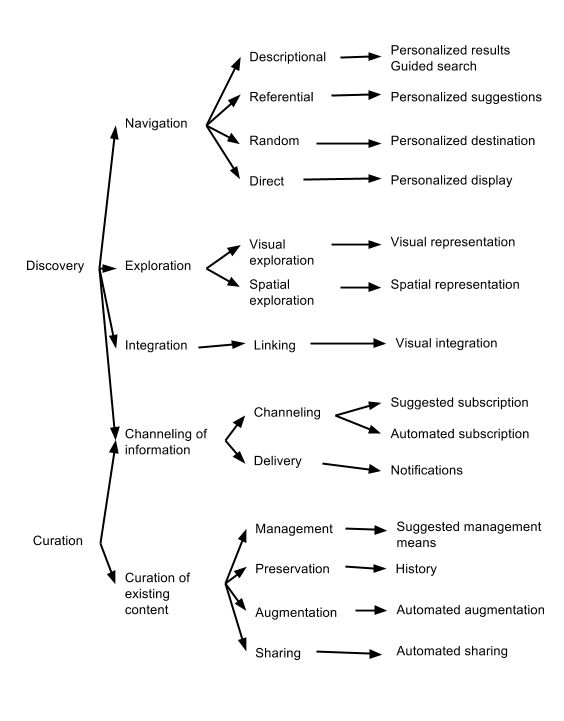
\includegraphics[width=\linewidth]{overview.png}
	\caption{Conceptual Framework Overview}
	\label{fig:overview} 
\end{figure}



{\section{Discovery and Navigation}
In order to discover information, a user needs to have a way of navigating to it. Common methods of navigation that facilitate information discovery include descriptional, referential, random, and direct (see Table~\ref{table:navigation}). 

\begin{table}[ht!]
\caption{Navigation Mechanisms}
\label{table:navigation} 
\begin{tabular}{{|p{0.35\linewidth}|p{0.60\linewidth}|}}
\hline
Navigation mechanisms     	& Questions to be posed during the design or evaluation of tools \\
\hline
\textbf{Descriptional} 			& \\
Search-based navigation 		& Can users navigate the site using search mechanism? \\
\textbf{Referential}       		& \\
Category-guided navigation 		& Can users navigate using categories? \\
Facet-guided navigation    		& Can users navigate using facets? \\
Filters-guided navigation  		& Can users navigate using filters? \\
Tag-guided navigation      		& Can users navigate using filters? \\
Search by resource         		& Can the user search by resource? \\
\textbf{Random}            		& \\
Random navigation          		& Is it possible to randomly navigate through resources? \\
\textbf{Direct}            		& \\
Direct display             		& Is any information displayed directly without active search? \\
\hline
\end{tabular}
\end{table}

{\subsection{Descriptional Navigation}
A navigation is descriptional when the user describes the information need. Most commonly is implemented as search-based navigation since it allows users to enter the search query and describe their information need.

There are two common ways of aiding information discovery when search-based navigation is used. The first method entails returning personalized results when the user enters a search query. There are a number of ways to accomplish personalization, but this chapter only focuses on which features can can support information discovery and curation have rather than their implementations. The second method is to suggest search terms to make it easier for the user to formulate the information need (see Table~\ref{table:navigation_support}). 

There exist numerous ways in which descriptional navigation supports information discovery. With fact discovery, an information need is known ~\cite{kellar2006, kellar2007}. Therefore, descriptional navigation provides a way of for the user to express her information need. 

Search-based navigation often serves as an entry point for information seeking ~\cite{levene}. In case of serendipitous discovery, since the information need is not well articulated, descriptional navigation can be used to express a topic that could potentially relate to the information need. For instance, searching for a location within Pinterest returns numerous images of the location that link to (or integrate with) other resources, blogs, and Web pages, whereas searching for the same place on Google Maps usually returns a small set of possible locations with limited information about those places.

Descriptional navigation can help rediscovering information. However, search-based rediscovery is not always a reliable way of refinding information ~\cite{cockburn}. In information portals that provide access to fairly ambiguous information and that have information regularly repopulated and updated, the search feature is usually designed around retrieving information related to some topic, but is not very specific. In order to revisit a resource, search must provide consistent results. In information discovery applications that provide access to specific information, such as Wikipedia and Rotten Tomatoes, search can usually lead directly to a specific resource. However, within Web applications such as We Heart It or Pinterest, search-based rediscovery is often unreliable.
} % end subsection

{\subsection{Referential Navigation}
A navigation is referential when the user finds a reference to the term that she is looking for.  The underlying assumption of this method of navigation is that the user can recognize needed information as she sees it.

Referential navigation methods can take many different forms. Some common ones are searching categories, facets, and filters. Often, Web applications implement tag-based navigation. In some applications, users can search by a given resource (see Table~\ref{table:navigation}).

To further support referential navigation, applications can either personalize search results (similarly to descriptional navigation) or personalize reference suggestions (see Table~\ref{table:navigation_support}). 

rentialRefe navigation is used to direct the user to relevant resources ~\cite{levene}. In the case of fact discovery, such navigation should narrow the results to a specific type of resource so that further fact discovery is bounded by that type. For example, TripAdvisor lets the user choose among flights, hotels, vacation rentals, restaurants, and destinations.

For serendipitous discovery, referential navigation should provide a way to narrow the results to those related to one topic. In addition, categories, facets, filters, and tags can help the user formulate an information need by suggesting topics ~\cite{levene}. For example, when using Google Images, every search query suggests related categories of images to help users define an information need.

} % end subsection

{\subsection{Random Navigation}
In order to browse diverse information, an information discovery tool needs to provide a way to randomly navigate among resources, thereby supporting serendipitous information discovery ~\cite{foster}. Many applications, such as StumbleUpon, support random navigation to allow for opportunistic jumping from one resource to another. This method is useful when the information need is undefined.

To further enhance random navigation, Web tools sometimes allow users to personalize this type of navigation, which makes it less 'random'. However, this way the user can discover new information within a specific category, for example.
} % end subsection

{\subsection{Direct Navigation}
In a broad sense of Web-based navigation, direct navigation is associated with entering an address of a site and being redirected directly to it. In the context of Web applications for information discovery, direct navigation means displaying certain content to the user without user's active participation.  

Often, applications display certain information as soon the user visits the site. It can be news feed, featured content, context-dependent information, or other types of information. Displayed content can also be personalized to improve information discovery with direct navigation.

} % end subsection

\begin{table}[ht!]
\caption{Automation and Support for Navigation}
\label{table:navigation_support}
\begin{tabular}{{|p{0.35\linewidth}|p{0.60\linewidth}|}}
\hline
Automation                   & Questions to be posed during the design or evaluation of tools \\
\hline
\textbf{Descriptional}       & \\
Personalized results         & Do the descriptional mechanisms return personalized results? \\
Guided search                & Is the descriptional mechanism guided by suggested search terms? \\
\textbf{Referential}         & \\
Suggesting topics of interest& Does the application suggest topics of interest? \\
Suggesting similar resources & Does the application suggest similar resources? \\
Suggesting tags              & Does the application suggest similar tags? \\
\textbf{Random}              & \\
Personalized destination     & Is random navigation personalized to the user? \\
\textbf{Direct}              & \\
Personalized display         & Is direct display personalized to the user? \\                                                       
\hline

\end{tabular}
\end{table}
} % end section

{\section{Exploration and Discovery}
Exploration of resources is another factor that enables information discovery. In particular, visual and spatial explorations of single or multiple resources allow for rapid information searching (see Table ~\ref{table:exploration}). 

Abrams et al.~\cite{abrams} identified link representation as one of the problems with traditional bookmarking. Analogous with browsing through a bookmark manager, identifying relevant information when browsing through links to diverse resources can be a challenging task. A visual preview should make it easier to evaluate the relevance of resources. Applications that facilitate serendipitous information discovery often employ elaborate resource representation techniques. Many social bookmarking systems, such as Scoop.it! and StumbleUpon, support visual previews of bookmarked pages. Delicious is a social bookmarking application that lacks this type of link representation support, which makes it harder to determine if the link will lead to a relevant resource.

Similar to link representation, spatial visualization of numerous links is another problem that occurs when browsing through diverse content ~\cite{abrams}. Therefore, a semantic to the spatial arrangement of resources is of major importance. Information discovery applications that support serendipitous discovery often have a special way of spatially arranging resources to make it easier to browse through large amounts of information. For example, many tools use a 'pinboard' layout of resources similar to Pinterest.

\textbf{Uniform representation.} Uniform representation is a method of displaying diverse resources in a common way, with each resource having the same set of components ~\cite{herrera}. Such a representation assures that each resource has the same set of facts associated with it, and therefore, the user can afford to have expectations about information that can be found when looking for a specific fact. For example, Yelp displays rating, price range, and address for all restaurants, so not only is it easy to find specific information, but the user can have expectations about the content of resources within the application. On the contrary, searching Tumblr for a restaurant will return a chaotic collection of information about the place. 



\textbf{Visual link preview.} If an application provides links to resources, a visual preview makes it easier to recognize the relevance of the resource ~\cite{abrams}. Applications that support fact discovery often use visual link preview, similar to applications that support serendipitous browsing. However, the motivation behind having a link preview for fact finding is to make it possible to identify if the resource is indeed what the user is looking for. For example, searching for an actor in IMDb will return a list of actors and their photographs, so that the user can pick the one they are interested in.

\textbf{Spatial arrangement.} Similar to serendipitous information discovery, spatial arrangement of resources is important ~\cite{abrams} as a poor semantic to the arrangement can make it difficult to visually navigate to the facts of interest.

\begin{table}[ht!]
\caption{Exploration Mechanisms}
\label{table:exploration}
\begin{tabular}{{|p{0.35\linewidth}|p{0.60\linewidth}|}}
\hline

Method of exploration                       & Questions to be posed during the design or evaluation of tools                                                    \\
\hline
\textbf{Visual exploration}                 &                                                                                       \\
Visual exploration of a single resource     & Does the system visual exploration of a single resource?                        \\
Visual exploration of multiple resources    & Does the system allow visual exploration of multiple resources? \\
\textbf{Spatial exploration}                &                                                                                       \\
Spatial exploration of a single resource    & Does the system provide means for spatial resource exploration?                       \\
Spatial exploration of a multiple resources & Does the system provide means for spatial exploration for multiple resources?        \\                                                       
\hline

\end{tabular}
\end{table}

\begin{table}[ht!]
\caption{Support for Exploration of Multiple Resources}
\begin{tabular}{{|p{0.35\linewidth}|p{0.60\linewidth}|}}
\hline
Method of exploration of multiple resources & Questions to be posed during the design or evaluation of tools  \\
\hline
\textbf{Visual exploration}                 &                                              \\
Visual preview                              & Are there visual previews of resources?      \\
Textual preview                             & Are there textual previews of resources?     \\
\textbf{Spatial exploration}                &                                              \\
List                                        & Are resources presented in a list?           \\
Grid                                        & Are resources presented in a list?           \\
Gallery                                     & Are resources presented in a gallery layout? \\
Consistent representation                   & Are resources presented in a consistent way?  \\                                                       
\hline

\end{tabular}
\end{table}

\begin{table}[ht!]
\caption{Support for Exploration of a Single Resource}
\begin{tabular}{{|p{0.35\linewidth}|p{0.60\linewidth}|}}
\hline
Method of exploration of single resource & Questions to be posed during the design or evaluation of tools \\
\hline
\textbf{Visual exploration}              & \\
Visual cues                              & Are there visual cues? \\
Textual cues                             & Are there textual cues? \\
\textbf{Spatial exploration}             & \\
Spatial semantic                         & Is there a semantic to the spatial arrangement of resources? \\
Consistent representation                & Are resources presented in a consistent way?\\                                                       
\hline

\end{tabular}
\end{table}
} % end section
{\section{Integration}

Similar to serendipitous discovery, if an information discovery application provides access to resources from other Websites, the user should be able to navigate to those sites as they may contain the facts of interest. Integration for fact finding is especially important when it gives an opportunity to display specific information about resources that otherwise would not be accessible. For example, Google Maps displays business ratings as a result of its integration with Google+.

To users with ambiguous information needs, one information portal might not provide access to all information of interest. If an information discovery application gives access to resources from various sources, such as other Websites, the user should be able to navigate back to those sources.  

\begin{table}[ht!]
\caption{Integration}
\begin{tabular}{{|p{0.35\linewidth}|p{0.60\linewidth}|}}
\hline
Integration mechanism  & Questions to be posed during the design or evaluation of tools \\
\hline
\textbf{Integration} &                                                    \\
Linking   & Is application linked to another application?\\                                                       
\hline

\end{tabular}
\end{table}

\begin{table}[ht!]
\caption{Support for Integration}
\begin{tabular}{{|p{0.35\linewidth}|p{0.60\linewidth}|}}
\hline
Integration support  & Questions to be posed during the design or evaluation of tools \\
\hline
\textbf{Integration} &                                                    \\
Visual integration   & Is another application's data visually integrated?\\                                                       
\hline

\end{tabular}
\end{table}
} % end section

{\section{Curation}

Information curation is a common activity within many information discovery applications. By asking questions about application design with regards to information curation as in Tables~\ref{table:curation} and~\ref{table:curation_support} of the conceptual framework, designers can find ways to add value to information and enable information exploitation over time.

Information discovery applications vary from being completely socially curated and populated by users, to those that lack any curation mechanisms. 
By definition, digital information curation is the notion of managing, preserving, and adding value to collections of information ~\cite{beagrie, wittaker}. Thus, the curation category consists of information management, preservation, information enhancement, and sharing.


\begin{table}[ht!]
\caption{Curation Mechanisms}
\label{table:curation}
\begin{tabular}{{|p{0.35\linewidth}|p{0.65\linewidth}|}}
\hline
Curation support  & Questions to be posed during the design or evaluation of tools  \\
\hline
\textbf{Management}                   &                                                                                                           \\
Collection-based categorization       & Does the application support sorting information into collection-like structures, either privately or publicly?                                                  \\
Tag-based categorization               & Does the application support tagging, either privately or publicly?                                                \\

\textbf{Preservation}                  &                                                                                                           \\
Internal preservation of internal resources       & Does the application support mechanism(s) for preserving internal information within the application?        \\
Internal preservation of external resources       & Does the application support mechanism(s) for preserving external information within the application?        \\
External preservation of internal resources      & Does the application support mechanism(s) for preserving internal information outside of the application? \\ 

\textbf{Augmentation}            &                                                                                                           \\
Evaluation                   & Can the resource evaluations be recorded privately or publicly? \\
Annotation                   & Can resources be annotated privately or publicly?                                                                               \\    
       
\textbf{Sharing}           &                                                                                                           \\
Adding resources             & Can resources be publicly added to the collection of information within the application from other Web pages?     \\
Internal sharing         & Can internal resources be publicly reshared within the application?         \\ 
External sharing          & Can internal resources be publicly reshared outside of the application?         \\ 
\hline        
\end{tabular}
\end{table}

\begin{table}[ht!]
\caption{Curation Support and Automation}
\label{table:curation_support}
\begin{tabular}{{|p{0.35\linewidth}|p{0.65\linewidth}|}}
\hline
Curation support  		& Questions to be posed during the design or evaluation of tools \\
\hline
\textbf{Management}		&                                                                                                           \\
Suggesting collections  & Does the application suggest relevant collections? \\
Suggesting tags         & Does the application suggests relevant tags? \\
\textbf{Preservation}   & \\
History       			& Does the application automatically preserve found information? \\
\textbf{Augmentation} 	& \\
Automatic augmentation  & Does the application automatically annotates resources? \\    
\textbf{Sharing}        & \\
Automatic sharing		& Are resources shared automatically? \\
\hline        
\end{tabular}
\end{table}


{\subsection{Management}
Information management is one of the key elements of information curation ~\cite{beagrie, wittaker}. Information categorization mechanisms are prevalent in applications that have a lot of information that is hard to categorize automatically or can mean something different for each user. In the context of Web information management, the following factors play a major role.

Resource categorization helps establish relationships between various resources ~\cite{beagrie, wittaker}. Allowing people to sort information using custom categories can aid rediscovery, discovery in a socially curated space, as well as add more value to resources.

Similar to list-based categorization, tagging aids rediscovery, adds value to resources, and aids discovery, especially in a socially curated space ~\cite{gruber}.  For example, Pinterest supports tag- and list-based categorizations, where lists are represented as 'pinboards'. Tumblr, on the other hand, only supports tag-based categorization. In addition, Pinterest allows for private information categorization.

} % end subsubsection

{\subsection{Information Preservation}
Information preservation is a common Web task that is usually performed with the intent of revisiting information ~\cite{abrams, wittaker}. However, in the case of opportunistic Web use, information gathering is sometimes performed with just the goal of collecting information rather than revisiting it in the future ~\cite{lindley}. Bookmarking is a traditional way of preserving information and many Web applications provide diverse bookmarking mechanisms. 

Internal preservation of internal resources means bookmarking resources to be reaccessed within the same application. Such bookmarking facilitates information curation within the system.

Internal preservation of external resources signifies bookmarking other Web pages within an application. 
  
External preservation means bookmarking resources so that they become available through other bookmarking systems. An application must facilitate integration with other applications in order to enable external preservation ~\cite{abrams}.

On We Heart It, users can preserve \textit{internal  information} using \textit{internal collections} and they can add information from \textit{external} Websites. However, there are no integrated means for bookmarking \textit{internal content} using other bookmarking systems.  


Bookmark-based revisitation is one of the most common ways of information rediscovery ~\cite{abrams}. The majority of Web browsers are equipped with bookmarking features. However, some modern Web applications, such as YouTube and Pinterest, provide integrated mechanisms for bookmarking and bookmark-based information rediscovery. 

A Web application needs to automatically record browsing history in order to enable history-based rediscovery ~\cite{tauscher}. History-based rediscovery appears to be the least common rediscovery mechanism, however, it can still be found in some Web applications, such as Google Maps.
} % end subsubsection

{\subsection{Augmentation}
One of the most important elements of digital curation is augmentation: adding value to information ~\cite{beagrie, wittaker}. It is often performed within social bookmarking systems. Many Web applications allow users to add value to the resources they curate. 

Evaluation methods can have various forms. They usually take place in socially curated information systems. However, evaluation can also contribute to personal reflection and information preservation. In addition, many applications allow users to evaluate resources by rating them or recording other forms of approval or disapproval. Some sites, such as Wikipedia, do not allow any evaluation. 

Annotations are metadata attached to a resource, such as comments and descriptions. Annotations make it easier to search for and interpret information. 
} % end subsubsection

{\subsection{Sharing}
Sharing information is key to empowering social information curation ~\cite{beagrie}. Therefore, the main components that facilitate sharing are adding resources, and external and internal information sharing.

Adding resources not only facilitates global Web information curation, but it also scales the information available through the system, providing more opportunities for information discovery. Resources can be created by users themselves, taken from some other sources online, or both. For example, YouTube allows users to upload their own videos, whereas Pinterest permits adding images from other sites in addition to users' personal images. 

Sharing resources through different media supports channel-based information discovery within the media channels. Information discovery applications commonly allow for sharing information on popular networking sites outside the application.

Resharing resources within the system supports channel-based information discovery. 
} % end subsubsection



} % end section


{\section{Channelled Curation and Discovery}

{\subsubsection{Channel-based Discovery}

Subscriptions to updates from a site help users follow the news ~\cite{java}. In order to support subscription-based discovery, an application must provide a subscription mechanism. For example, Rotten Tomatoes allows subscriptions to newsletters; however, it does not allow subscriptions to movie critics, as a user-based subscription mechanism would allow. 

In some applications, the content is updated and curated by users, and users can subscribe to other users. Similar to site subscriptions, user subscriptions are subscriptions to activity updates from individual users rather than all content updates, and help with networking and following users' activities ~\cite{millen}. Such subscriptions help to further filter new content delivered to the user. 

Notification mechanisms enable user awareness about new content on the subscribed channel ~\cite{millen}. Different applications provide various notification mechanisms including messages within the application, informative emails, and smartphone notifications.

Displaying a news feed within the application further promotes awareness and can serve as a monitoring mechanism. For such. 

Similar to displaying a subscription news feed, displaying a content news feed promotes awareness and can serve as a monitoring mechanism.

Information discovery tools can have different implementations depending on the purpose of discovery. Using the information discovery factors in our framework (see Table 2), we described and evaluated currently existing tools. Similarly, the framework can be used for identifying gaps in information discovery support and developing new technologies (see Sec. 5).   \\

} % end subsubsection

\begin{table}[ht!]
\caption{Chenneling Mechanisms}
\begin{tabular}{{|p{0.35\linewidth}|p{0.60\linewidth}|}}
\hline
Channelling mechanisms     & Questions to be posed during the design or evaluation of tools \\
\hline
\textbf{Subscriptions}     &                                                         \\
User subscription          & Can the user subscribe to activities of other users?    \\
Site subscription          & Can the user subscribe to site updates?                 \\
Artifact subscription      & Can the user subscribe to artifact updates?             \\
\textbf{Notifications}     &                                                         \\
User activity overview     & Does the application display activities of other users? \\
Site activity overview     & Does the application display site updates?              \\
Artifact activity overview & Does the application display activities of other users?\\                                                       
\hline

\end{tabular}
\end{table}

\begin{table}[ht!]
\caption{Channeling Support}
\begin{tabular}{{|p{0.35\linewidth}|p{0.60\linewidth}|}}
\hline
Channeling support               & Questions to be posed during the design or evaluation of tools \\
\hline
\textbf{Subscriptions}            &                                                                    \\
Suggesting users                  & Are users suggested to the user?                                   \\
Automatic subscription            & Can the system subscribe the user automatically?                   \\
Suggesting artifacts              & Are artifacts suggested to the user?                               \\
\textbf{Notifications}            &                                                                    \\
User activity update notification & Does the application display activities of other users?            \\
Site activity update notification & Does the application notify the user about site updates?           \\
Artifact update notification      & Does the application notify the user about updates on an artifact?\\                                                       
\hline

\end{tabular}
\end{table}

} % end section














\chapter{Improving Information Discovery and Curation Activities}
\label{chapter:improving}



\begin{table}[ht!]
\caption{Automation and Support for Navigation}
\label{table:navigation_support}
\begin{tabular}{{|p{0.35\linewidth}|p{0.60\linewidth}|}}
\hline
Automation                   & Questions to be posed during the design or evaluation of tools \\
\hline
\textbf{Descriptional}       & \\
Personalized results         & Do the descriptional mechanisms return personalized results? \\
Guided search                & Is the descriptional mechanism guided by suggested search terms? \\
\textbf{Referential}         & \\
Suggesting topics of interest& Does the application suggest topics of interest? \\
Suggesting similar resources & Does the application suggest similar resources? \\
Suggesting tags              & Does the application suggest similar tags? \\
\textbf{Random}              & \\
Personalized destination     & Is random navigation personalized to the user? \\
\textbf{Direct}              & \\
Personalized display         & Is direct display personalized to the user? \\                                                       
\hline

\end{tabular}
\end{table}


\begin{table}[ht!]
\caption{Support for Exploration of Multiple Resources}
\begin{tabular}{{|p{0.35\linewidth}|p{0.60\linewidth}|}}
\hline
Method of exploration of multiple resources & Questions to be posed during the design or evaluation of tools  \\
\hline
\textbf{Visual exploration}                 &                                              \\
Visual preview                              & Are there visual previews of resources?      \\
Textual preview                             & Are there textual previews of resources?     \\
\textbf{Spatial exploration}                &                                              \\
List                                        & Are resources presented in a list?           \\
Grid                                        & Are resources presented in a list?           \\
Gallery                                     & Are resources presented in a gallery layout? \\
Consistent representation                   & Are resources presented in a consistent way?  \\                                                       
\hline

\end{tabular}
\end{table}


\begin{table}[ht!]
\caption{Support for Exploration of a Single Resource}
\begin{tabular}{{|p{0.35\linewidth}|p{0.60\linewidth}|}}
\hline
Method of exploration of single resource & Questions to be posed during the design or evaluation of tools \\
\hline
\textbf{Visual exploration}              & \\
Visual cues                              & Are there visual cues? \\
Textual cues                             & Are there textual cues? \\
\textbf{Spatial exploration}             & \\
Spatial semantic                         & Is there a semantic to the spatial arrangement of resources? \\
Consistent representation                & Are resources presented in a consistent way?\\                                                       
\hline

\end{tabular}
\end{table}



\begin{table}[ht!]
\caption{Support for Integration}
\begin{tabular}{{|p{0.35\linewidth}|p{0.60\linewidth}|}}
\hline
Integration support  & Questions to be posed during the design or evaluation of tools \\
\hline
\textbf{Integration} &                                                    \\
Visual integration   & Is another application's data visually integrated?\\                                                       
\hline

\end{tabular}
\end{table}

\begin{table}[ht!]
\caption{Curation Support and Automation}
\label{table:curation_support}
\begin{tabular}{{|p{0.35\linewidth}|p{0.65\linewidth}|}}
\hline
Curation support  		& Questions to be posed during the design or evaluation of tools \\
\hline
\textbf{Management}		&                                                                                                           \\
Suggesting collections  & Does the application suggest relevant collections? \\
Suggesting tags         & Does the application suggests relevant tags? \\
\textbf{Preservation}   & \\
History       			& Does the application automatically preserve found information? \\
\textbf{Augmentation} 	& \\
Automatic augmentation  & Does the application automatically annotates resources? \\    
\textbf{Sharing}        & \\
Automatic sharing		& Are resources shared automatically? \\
\hline        
\end{tabular}
\end{table}


\begin{table}[ht!]
\caption{Channeling Support}
\begin{tabular}{{|p{0.35\linewidth}|p{0.60\linewidth}|}}
\hline
Channeling support               & Questions to be posed during the design or evaluation of tools \\
\hline
\textbf{Subscriptions}            &                                                                    \\
Suggesting users                  & Are users suggested to the user?                                   \\
Automatic subscription            & Can the system subscribe the user automatically?                   \\
Suggesting artifacts              & Are artifacts suggested to the user?                               \\
\textbf{Notifications}            &                                                                    \\
User activity update notification & Does the application display activities of other users?            \\
Site activity update notification & Does the application notify the user about site updates?           \\
Artifact update notification      & Does the application notify the user about updates on an artifact?\\                                                       
\hline

\end{tabular}
\end{table}
\chapter{Framework Application for Design}
\label{chapter:application}

To verify that the conceptual framework is effective, I applied it to design a place photo discovery application. This chapter outlines the role the framework played in the design process of the Web application, the resulting application and its features, and some prospects for future application development. 

{\section{Applying the Conceptual Framework to Design an Application}
A need for a place photo discovery application was revealed during the construction phase of the framework. Asking questions from the preliminary framework (see Chapter~\ref{chapter:old_framework}) about existing applications, such as Pinterest and Google Maps, helped expose the need for discovery and curation of place photos with additional access to place location data and other details. It also helped gather some of the requirements for a photo discovery application.

In general, Web applications that are tailored towards image discovery, such as Pinterest and We Heart It, support user's motive to close a knowledge gap that is characterized by underdefined information need. To deal with the issue of having an underdefined information need, an application has to help the user to formulate their information need as well as support serendipitous discovery of information. In order to enable serendipitous discovery, Web applications regularly update the content they provide by allowing users to add new resources and curate information. 

The task of image seeking for the purpose of finding inspiration (as it is the case for the majority of Pinterest users) can stretch out to multiple sessions over an undetermined period of time. Curation mechanisms, such as preservation and management, help rediscover information to reflect on the previous findings and continue the task.  

It is common for users to discover place photographs on Pinterest, and Pinterest does display a map when a location of a place is known within the system. However, this feature only applies to a relatively small fraction of existing `pins'. In addition, Pinterest facilitates discovery of images related to diverse topics and interests, and not only places, which makes it harder to tailor user experience to facilitate discovery and curation based on the desired motives. 

When it comes to place discovery, the Google Maps application provides the ultimate support for finding place and business locations. It is also possible to see what a place looks like based on associated image. However, since the application is oriented towards finding specific information, visual and spatial photo exploration mechanisms are not well-developed. The user can preserve a given place but cannot preserve or organize photographs of places. Google Maps also lacks category-based navigation mechanisms which can help defining an information need.  

The findings above helped me define a motive for a place photo discovery application, which is to find inspirational (underdefined) place photographs, to collect and manage found information for future use and retrieval, as well as to provide access to more defined information about the place, such as its location. After formalizing the motive for the application use, I referred back to the framework to choose options for supporting various aspects of information discovery and curation while developing the application.
}

{\section{KeePlaces and Its Features}
The resulting application, KeePlaces\footnote[1]{A prototype of KeePlaces is available at www.keeplaces.com}, supports discovery and curation of place photographs, and it is integrated with Google Maps. This section outlines the main features of KeePlaces in accordance with the conceptual framework. 

Descriptional navigation is possible using search. The search feature is not guided, and so far, results are not personalized. 


Spatial exploration of multiple resources is enabled through the gallery view. 
Resources are represented as photos, so visual exploration of multiple resources is enabled. However, there is no way of exploring each resource individually, therefore, exploration of a single resource is not supported. 

KeePlaces is integrated with Google Maps.

Curation in Keeplaces is supported through management and preservation.

Management is implemented using collection-based classification.
Every photo discovered on the site can be bookmarked, or 'kept', in a collection.

Channeling has not yet been enabled within the application, but it is an important aspect behind the conceptual model of the application.


\begin{figure}[ht!]
	\noindent
	\centering
	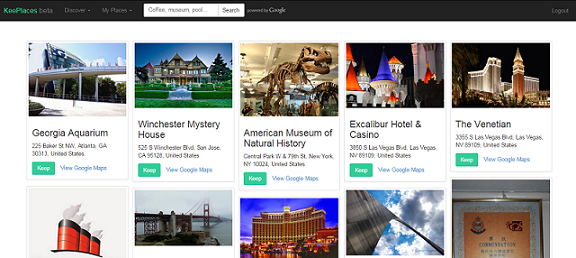
\includegraphics[width=\linewidth]{keeplaces.png}
	\caption{KeePlaces Interface}
	\label{fig:keeplaces} 
\end{figure}
}
{\section{Directions for Future Development}
As mentioned above, channeling is the first aspect that needs to be implemented along with enhancing management mechanisms.

} % end section

{\section{Discussion}


} % end section





\chapter{Research and Design Implications}
\label{chapter:implications}

The conceptual framework for information discovery and curation is designed to perform formative and summative evaluation of existing Web applications, with a goal to reveal how these tools support information-related activities in question. The framework, as a tool, and its capability to guide the process of analyzing Web applications makes it broadly applicable in research and Web design. 

In Chapter~\ref{chapter:evaluation}, I demonstrate how the framework can be used to reveal missing features in tools. Using similar methods, the framework can also be applied to compare different Web applications. When used for evaluation, the framework helps to identify which areas of a given tool require further attention. Therefore, the framework can be helpful for designers who wish to improve existing tools or get ideas for new information discovery and curation applications. 

Factors and questions of the framework are there to guide the developer, but they do not dictate which features should be in an application. In other words, the framework helps expose gaps, but it is up to designers to decide whether those gaps need to be closed. In fact, some gaps cannot be closed because of certain constraints, such as data type and system design.

User interface designers face certain trade-offs when developing applications. Therefore, it is not always advantageous to implement all of the missing features. For example, providing the tools to customize spatial arrangement of multiple resources can undermine the consistency of their representation. 

In the research domain, the framework can serve as a guide for drawing distinctions between different Web-based information discovery and curation applications, finding gaps in tools that can be studied, and selecting cases for studies based of required functionality. Hence, both researchers and developers can benefit from the systematic tool examination guided by the framework.

Even though applying the framework requires initial expertise and critical reasoning, it opens up opportunities for research and Web design. Systematic evaluation of Web tools for information discovery and curation gives the power to improve user experience and to gain better understanding of information behaviour within a given system. 





\chapter{Future Work and Conclusions}
\label{chapter:future_work}


In my study, I analyzed information curation and seeking tasks and developed a conceptual framework of factors and questions that are important when building and evaluating Web information discovery and curation tools. I then evaluated and iteratively refined the framework by analyzing 20 different information discovery applications and provided concrete examples of tool support addressing various concepts of the framework. Finally, I designed a Web-based application for place photo discovery and curation using the conceptual framework, and validated the framework by reevaluating five of the previously examined tools.

The current version of the framework is generalized to be applicable to most information discovery applications. Finding ways to instantiate the framework and extend it for use in domain-specific practices could serve as a potential future research goal. For example, video discovery and curation activities have unique properties related to the type of data to be discovered---information is mostly found in the video itself, and it cannot be viewed all at the same time. Hence, the framework could be extended to address domain-specific challenges. 

Another potential research direction would be to expand my investigation to include factors that influence the need for one information discovery type over another and further deepen an understanding of the relationships between the motives for information discovery and curation activities and information discovery types. 

\pagebreak
Additionally, one could investigate how collaboration in information discovery and curation relates to the conceptual framework. Generally, collaboration mechanisms in most Web information discovery applications are limited to information sharing, public information augmentation and tagging. However, collaboration often involves other activities, such as communication, coordination, and other domain-specific shared activities.

My framework opens up opportunities for structured information discovery and curation tool evaluation and design. As more tools are being developed within the social space of information discovery and curation, understanding how these tasks can be supported promises advancements in how Web applications are designed.







\bibliographystyle{apa}
\bibliography{refs}

\appendix              %- maybe some appendices
%\include{app1}
%\include{app2}

%--------------------------------------------------------------
%- Here is a semi-automatic VITA page construction.
%- If you don't like the page layout you have to make your own.
%--------------------------------------------------------------

\vita                  %- This commands starts the vita page(s)

%- Now call \fullinfo with four arguments:
%-    lastname, givenname, birthplace, and birthdate.
%- I think that the birthdate is according to Dec. 1994 rules
%-    is optional.
%- So, I also provide the command:
%-    \halfinfo{lastname}{givenname}{birthplace}


\halfinfo{Voyloshnikova}{Elena}{Nikolaev}

%-
%- Next, the education:
%- \begin{education} ... \end{education}
%- Each entry must be entered as \entry{university}{years}}
%-

\begin{education}
\entry{University of Victoria}{2008 to 2012}
\end{education}

%-
%- Next the degrees:
%- \begin{degrees} ... \end{degrees}
%- Now \entry has 3 arguments: \entry{title}{university}{year}
%-

\begin{degrees}
\entry{B.Sc.}{University of Victoria}{2012}
\end{degrees}

%-
%- Next the awards:
%- \begin{awards} ... \end{awards}
%- Entries look like: \entry{award}{year}
%-

\begin{awards}
\entry{award}{date}
\end{awards}

%-
%- Now the publications.
%- I broke it 3 parts: journal, conference, and `submitted_to'.
%- Use as:   \begin{jpubs} \item ... \item ... \end{jpubs}
%-           \begin{cpubs} \item ... \item ... \end{cpubs}
%-           \begin{spubs} \item ... \item ... \end{spubs}
%- Example:
%-

%\begin{jpubs}
%\item V.V. Dimakopoulos, G. Sourtziotis, A. Paschalis and D. Nikolos,
%   ``On TSC Checkers for $m$-out-of-$n$ Codes'',
%   {\it IEEE Transactions on Computers\/},
%   Vol.\ 44, No.\ 8, pp.\ 1055--1059, Aug.\ 1995.
%\item Another one, ...
%\end{jpubs}

%\begin{cpubs}
%\item V.V. Dimakopoulos and N.J. Dimopoulos, ``Optimal Total Exchange
%   in Cayley Graphs'', {\itshape submitted to\/} SIAM Journal on
%   Computing.
%\end{cpubs}

%\begin{spubs}
%\item V.V. Dimakopoulos and N.J. Dimopoulos, ``Optimal Total Exchange
%   in Cayley Graphs'', {\itshape submitted to\/} SIAM Journal on
%   Computing.
%\end{spubs}


%--------------------------------------------------------------
%- We can also produce the copyright and the withhold page.
%- These pages are unnumbered and should be printed at the
%- end. To construct the withhold page we need to know when
%- the successful defence was held. Also need the date for
%- the copyright page.
%--------------------------------------------------------------

\makecopyrightpage{30 Dec 2002}   %- Date below signature
%\makewithholdpage{30 Jan 2002}  %- When we defended

\end{document}
